\documentclass[11pt]{article}
\usepackage[a4paper,landscape,margin=0.72in]{geometry}
\usepackage[T1]{fontenc}
\usepackage{lmodern}
\usepackage{amsmath}
\usepackage{graphicx}
\usepackage{hyperref}
\title{Nonbranch weighted-Proj stalk: checked local boundary}
\author{Formal proof packet}
\date{28 October 2026}
\begin{document}
\maketitle
\noindent This report records a checked theorem and its explicit hypotheses. It adds no experiment, target result, or cost ratio. The editable SVG, standardized CSV, Lean source, and compiler log accompany this PDF.

\section*{Checked statements}
For any field $K$, quintic $f(x)=x^5+a_3x^3+a_2x^2+a_1x+a_0$, and rational pair $(a,y)$ with $y^2=f(a)$, the Lean file constructs the point on the actual weighted $\operatorname{Proj}$ curve through its $Z$ basic open. The theorem \texttt{pointProjStalkIso} identifies its structure-sheaf stalk with the affine coordinate-ring localization at the evaluation kernel. If $y\ne0$, \texttt{pointY\_unit} proves the pulled-back affine $y$ is a unit in that stalk.

The theorem \texttt{point\_norm\_order} is checked on this actual stalk \emph{with explicit} \texttt{IsDomain} and \texttt{IsDiscreteValuationRing} instances, and with $2$, $B$, and $y$ units, $N-By$ a nonunit, and $(N-By)(N+By)=u_1u_2U$. It concludes
\[
  \operatorname{ord}(N-By)=\operatorname{ord}(u_1)+\operatorname{ord}(u_2)+\operatorname{ord}(U).
\]
This applies the previously checked abstract local norm-order lemma; it does not discharge the DVR or formula-specific norm premises.

\section*{Verification and open gates}
Direct compilation with pinned Lean 4.34.1 exited zero. The pinned Mathlib revision is
\par\noindent\texttt{d13f23b723b8a846827a245b89c10fc7d3f11612}.
Seven printed theorem audits list only \texttt{propext}, \texttt{Classical.choice}, and \texttt{Quot.sound}; no \texttt{sorryAx}. Lean source SHA-256 is
\par\noindent{\small\texttt{3aca729afb11cdbf3992dc3db727b8d531922ecf381c423bc6bb6b2d6c3d3910}}.

The affine odd-quintic domain proof, principal nonbranch maximal ideal, and actual DVR instance remain open. So do transport of the proof-side common 2+2 numerator and norm factorization, a global principal divisor, $\mathrm{Pic}^0$ class transport, and compiled Rust semantics. The exact row-by-row status is in \texttt{nonbranch-stalk-order.csv}. Stalk transport follows the open-immersion principle in \href{https://stacks.math.columbia.edu/tag/01HD}{Stacks Project Tag 01HD}; the proposed local DVR criterion is \href{https://stacks.math.columbia.edu/tag/00PD}{Tag 00PD}.

\clearpage
\section*{Proof dependencies and gates}
\begin{center}
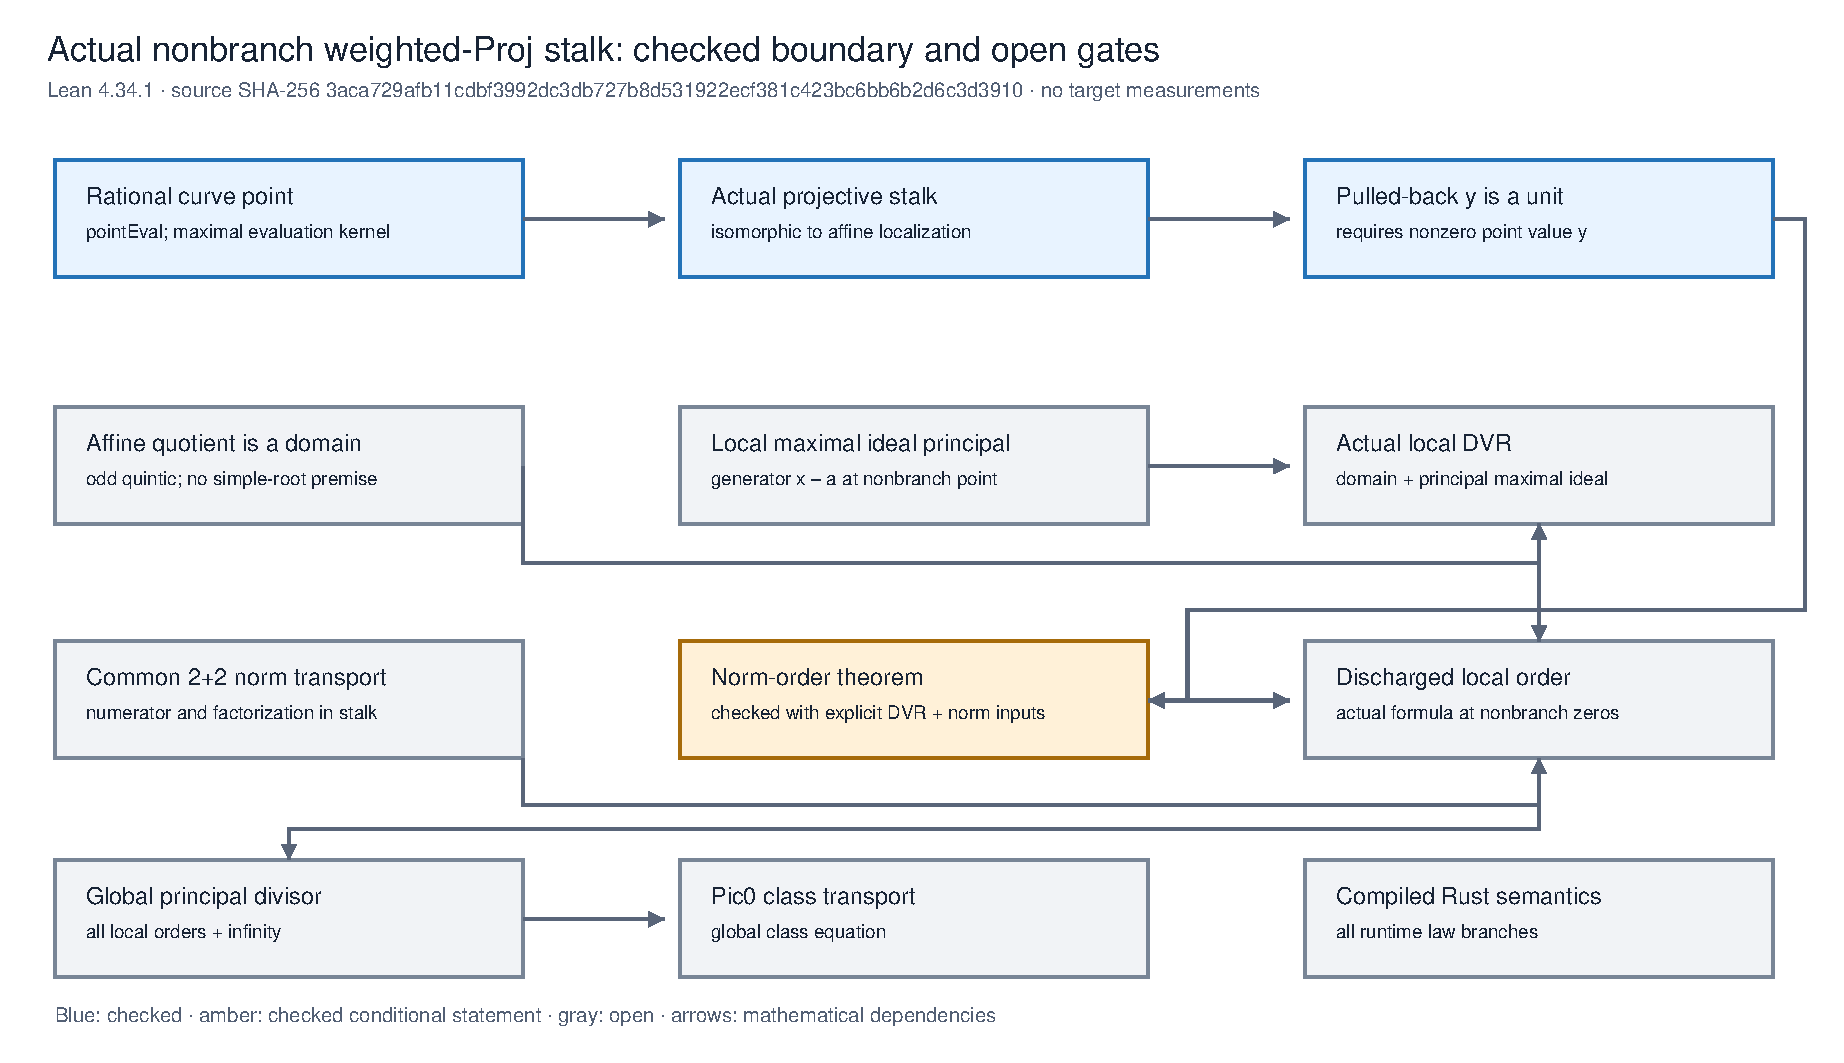
\includegraphics[width=0.96\textwidth,height=0.76\textheight,keepaspectratio]{nonbranch-stalk-order-figure.pdf}
\end{center}
\noindent Blue: checked; amber: checked conditional statement; gray: open. Arrows are proof dependencies. The diagram contains no performance data.
\end{document}
